\chapter{Image analysis}\label{sec:image-analysis}
\begin{remark}{Outline}
The scope of image analysis is wide and continually developing. Many of the advances in tools and techniques have evolved from the fields of biomedical imaging. Image analysis is central to many scientific methods, particularly where microscopy is concerned, therefore techniques are well established. Imaging methodologies for other life sciences, such as agriculture and ecology have not been as widely report on although this situation is changing as the hardware tools and software methods are becoming increasingly more powerful. Open source technologies are vital since many of the developments within the field of image analysis has depended on, or contributed towards reproducible scientific methods. Segmentation tools are key to most imaging tasks and methods have traditionally depended on high quality, laboratory acquired photography. This is no longer the case as it is now possible to quantify a range of digital images using new algorithmic machine learning methods, and interactive segmentation techniques. A review of some key aspects of image analysis theory and design are outlined in the following Chapter, with an emphasis on the practical tools and methods used in developing a generic image analysis system. The literature is discussed with the context of an image-centric method to monitor New Zealand's native bees using images of active nests.
\end{remark}

\section{Imaging and scientific discovery}\label{sec:imaging-and-scientific-discovery}
Science and photography have a close interdependent history dating back to the \emph{heliographic} experiments of the 1820's \cite{Delaney2008}. Imaging technologies are continuing to develop rapidly; according to the observations made by Moore the performance of hardware tools roughly doubles each year \cite{Bell2009}. The capabilities of modern imaging systems are remarkable as they are now integrated into everyday technologies such as cellular phones and laptop computers. Within the scientific domain sophisticated digital imaging systems are contributing to all manner of discoveries. From the intricate workings of the human brain in Single Photon Emission Computed Tomography imaging systems, \cite{Amen2011} to mapping the universe with the billion-pixel camera on the space probe Gaia \cite{Mignard2007}. The scope of image analysis is wide and it includes many distinctive strands of knowledge that have coalesced to form the current theory (Table \ref{tab:Imagea_scope}).

\begin{table}[!htbp]\myfloatalign \caption[Image analysis scope and topics.]{Image analysis scope and topics.}\label{tab:Imagea_scope} 
\begin{tabular}{p{1.4in}p{3.0in}}\toprule
Field of discipline & Main tasks \\ \midrule
Image processing:& Designing or applying filters or operators that change the basic aspects of an image (i.e. enhancing contrast and brightness). \\
Pattern recognition:&  Designing or applying the algorithms/code to automatically identify patterns in data.\\
Computer vision:& A complete system design -- from image acquisition to analysis (i.e robotic vision in manufacturing processes). \\
Machine learning:& Designing or applying the algorithms used in  semi-supervised/supervised machine learning scenarios.\\
Data-mining:& scanning for patterns that emerge from analysis of large quantities of data to help knowledge discovery.\\ \bottomrule 
\end{tabular}
\end{table}

The most comprehensive reviews regarding imaging methods are often directed towards biomedical image analysis. Microscopy is one of the fundamental tools of biology and traditionally scientists relied on visual interpretations of microscopic images. Consequently many advances towards automated imaging and analysis has been developed by and for biologists. Ljosa and Carpenter \cite{Ljosa2009} described a range of techniques used in imaging systems for the automated image analysis of microscopy images. \marginpar {Overview of quantitative analysis of microscopy images.} They presented a clear overview of current methods, providing a list imaging resources; they also outlined the pitfalls to consider when using or designing a quantitative imaging systems \cite{Ljosa2009}. Across disciplines image-tasks and pipelines are generally similar, therefore Ljosa and Carpenters' \cite{Ljosa2009} \marginpar{Pattern recognition software and techniques for biology.} manuscript provides some useful theory for other imaging research. Similarly two other  reviews, the first by Sharmir et. al. and second by Antony et. al.,  are equally informative; providing summaries of current software tools and techniques for life science image research \cite{Shamir2010,Antony2013}.

A handful of reviews are written for other areas of life science disciplines. For example, Pennekamp and Schtickzelle \cite{Pennekamp2013} \marginpar{A guide to implementing image analysis for ecology and evolution.} presented a hands on guide for imaging techniques in experimental laboratory systems. They introduced past, present and future benefits of technology with an overview of methodologies for experimental laboratory systems, explaining "...despite the advantages of image analysis, the technology has not been fully adopted yet, presumably due to the difficulties of technical implementation." \cite[pg.485]{Pennekamp2013}. They pointed out the range of benefits that could arise if automated image analysis and experimental laboratory systems were integrated. Imaging techniques can provide a fast reliable and low cost method to increase in the data for analysis in a range of biological parameters.

Gaston and O'Neill \cite{Gaston2004} reviewed imaging systems for pure and applied biology \marginpar{Automated species identification systems for biology.} and questioned the reasons why automated species identification has not been widely adopted. They investigated the core issues to determine if automated species identification would be a realistic option looking towards the future. They addressed the suggestions that the tasks are too difficult, too threatening, too different or too costly. Overall they concluded that "...vision and enterprise are more limiting...rather than the practical constraints of technologies." \cite [pg.1]{Gaston2004}.

\subsection{Image systems workflow}
Image analysis workflows consist of two major steps, image acquisition (capturing digital images) and image analysis (manipulating and measuring digital image data). These are generic stages across all methods, and disciplines. Glasbey and Horgan \cite{Glasbey1995} describe five distinct stages of images analysis as listed below. These are expanded in Figure \ref{fig:general-stages}.

\begin{itemize}
\item \emph{Acquisition and display}:  Capturing raw digital images; viewing an array of pixel values as an image on a digital camera or computer monitor.
\item \emph{Pre-processing}: Enhancing images by applying filter transformations to groups of pixels.
\item \emph{Segmentation}: Dividing an image into regions by sectioning or classifying pixels into different areas of objects.
\item \emph{Post-processing}: Applying operators that relate to the size and shape characteristics of objects to extract information from images.
\end{itemize}

\begin{figure}[!htbp] \myfloatalign
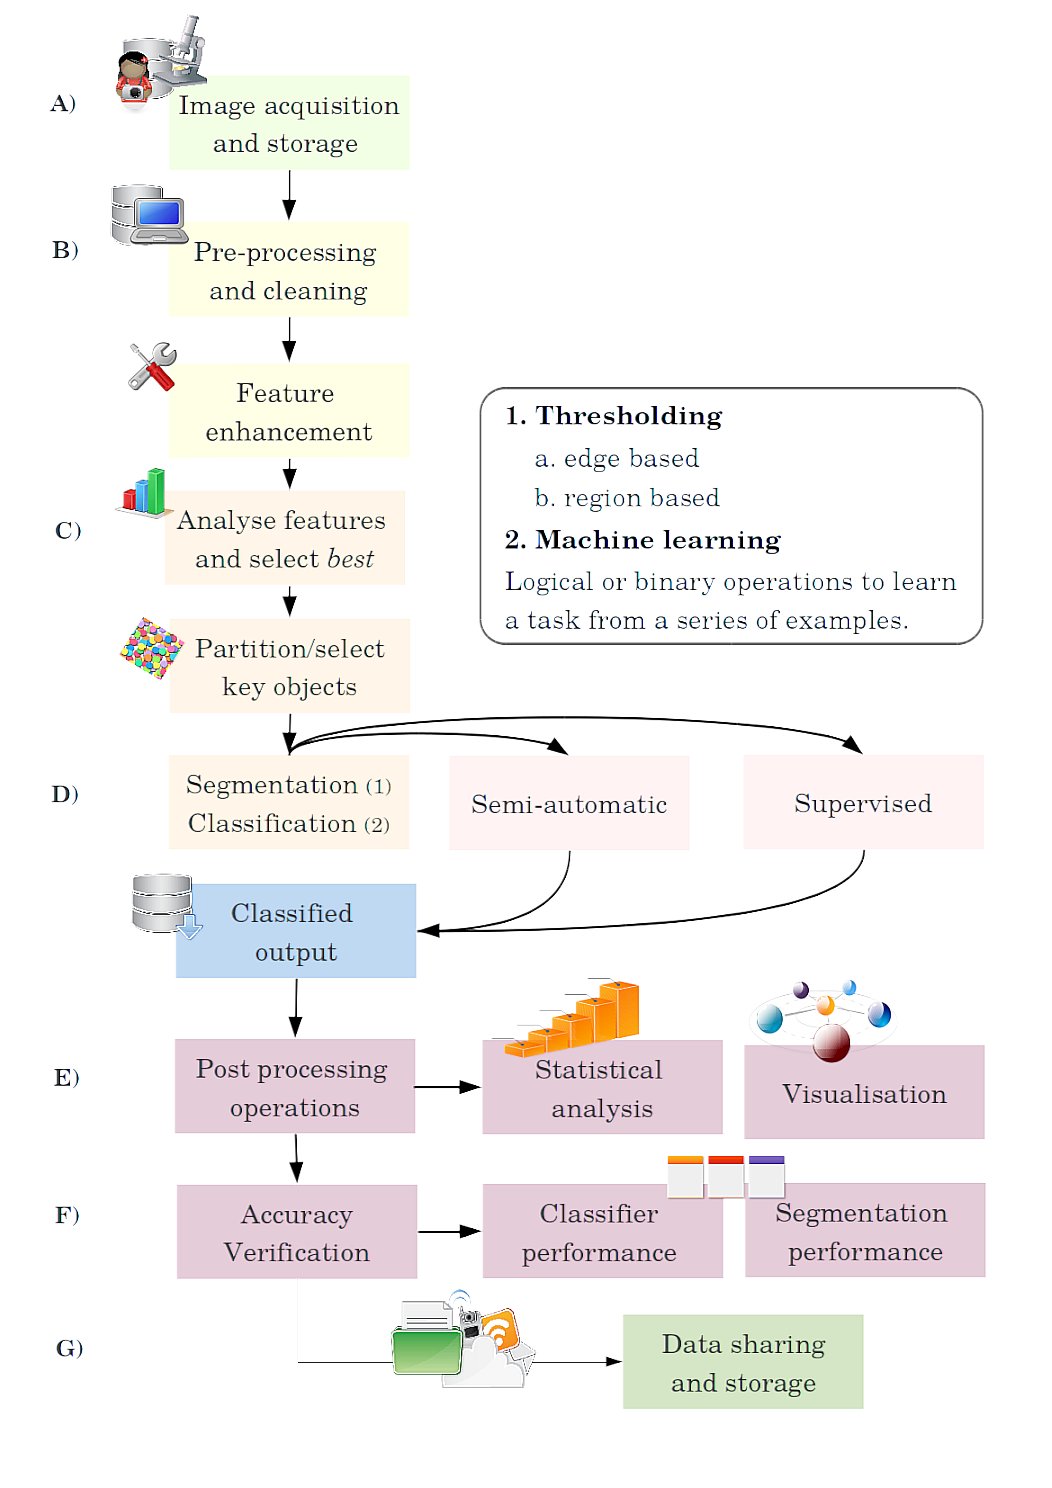
\includegraphics[width=1\linewidth]{gfx3/imagea_stages1}\\
\caption[Typical image analysis stages and design.]{Typical image analysis stages and design.}\label{fig:general-stages}
\end{figure}

Within medical imaging fields great attention is placed on the fidelity of raw image data, particularly with regards to method replication \cite{Pearson2007}. Guidelines on the appropriate use and manipulation of scientific digital images were presented by Cromey \cite{Cromey2010}. They are broadly relevant to other scientific imaging applications, although some points are not practically possible when collecting natural outdoor images (see points 4.* and 5.**).

\begin{enumerate}
\item Manipulation of digital images should only be performed on a copy of the unprocessed image data file.
\item Simple adjustments to an entire image is usually acceptable.
\item Cropping an images is usually acceptable.
\item Digital images that will be compared to one another should be acquired under identical conditions*, and any post-acquisition image processing should also be identical.
\item Avoid the use of lossy compression.**
\item Use care when changing the size (in pixels) of digital images.
\end{enumerate}

\subsection{Open-source tools}
The advances in electronic hardware tools and technologies have impacted the developments within the fields of image analysis. Off-the-shelf digital cameras are increasingly more powerful and parallel the advances in computers and imaging software tools. Increasing public access to technologies is changing much of the scientific landscapes, since the tools and methods are often readily available, easy to use, open-access and open-source.

For instance, although there are many good proprietary platforms available, open source software solutions are very popular and continue to be at the centre of many scientific advances. For example, Antony et al. \cite{Antony2013} reviewed imaging software tools and found open source packages offered substantial benefits, particularly with regards to reproducibility of methods \cite{Schindelin2012,Bouckaert2010weka}. \marginpar{Open-source, community driven image systems for biology.} More generally, the importance of open access was declared by a group of Nobel laureates; they explained that open access "...expands shared knowledge across scientific fields, it is the best path for accelerating multi-disciplinary breakthroughs in research." \cite{Openaccess}. 

Open source tools, methods, and open-access reporting can work in unison to advance the scientific knowledge \cite{Sonnenburg2007}. The versatility of software tools, access to code, and replication of methods are important factors that are worth considering during research design. As Antony et al. \cite{Antony2013} explain, " open-source solutions facilitate community--driven efforts in the development of image analysis " \cite[pg.13]{Antony2013}. The extendibility, interoperability, scalability of software platforms are key factors that have an impact on overall research methodologies. These are defined as:

\begin{enumerate}
\item Expandability: A system design principle taking future growth into consideration.
\item Interpolatable: The capability of different programs to exchange data using a common set of formats (to read and write the same in the same formats) and to use the same protocols, present or future, without any restricted access or implementation.
\item Scalability: The ability of a system, network, or process to handle a growing amount of work in a capable manner or its ability to be enlarged to accommodate that growth.
\end{enumerate}

Fiji \cite{Schindelin2012} is a popular biomedical imaging toolbox that has been carefully designed to consider all three factors listed. However, there are other packages commonly used for image analysis including: ImageJ \cite{Schneider2012}, Icy\footnote{Icy: {http://icy.bioimageanalysis.org/about}}\cite{De2012}, the Matlab plus Image Processing Toolbox \cite{Qidwai2011} and R--EBImage package \cite{Pau2010}.

\section{Image acquisition, format and pre-processing}
Digital image acquisition, formats and pre-processing methods are important aspects of image pipeline design. In biomedical imaging fields great attention is placed on the fidelity of raw image data, particularly with regards to method replication \cite{Pearson2007}. Final decisions can have cumulative impact on the integrity and analysis of image data, the validity of results and the reach of scientific outcomes. The quality and consistency of image capture is dependent on the acquisition methods. Under laboratory conditions important factors can be controlled such as lighting (i.e. brightness and background illumination) and the total capture area. Because there is greater control over image acquisition, the quality and reliability of image data and analysis is more measurable and methods are easier to replicate \cite{North2006}.

Natural images are complex and it is not possible to achieve the same degree of control when imaging under natural outdoor situations. Even so, a number of techniques can be used to help standardise acquisition. For example, Burks et al. \cite{Burks2000} used image analysis for agricultural monitoring to identifying different types of weeds. They designed a specialised image acquisition system to capture field images. They used a wheel mounted self contained imaging device which included four adjustable flood lights with diffuser covers to eliminate shadows \cite{Burks2000}. They described the variable natural conditions which affected image acquisition saying "...the combination of windy conditions with partly cloudy skies produced rapid changes in ambient light conditions and created significant leaf movement " \cite[pg.444]{Burks2000}. They explained that in order to reduce the affect of changing conditions, a diffuse off-white cotton cover was placed over the camera system, with supplemental lighting to compensate for the effects of cloud cover and angle of sun. A nylon canvas was also used as a wind break at the base of camera system to prevent excessive motion in the plant leaves \cite{Burks2000}. 

Over the last decade image acquisition techniques and analysis for agriculture have advanced considerably. For example \acp{UAV} are now used to capture hyper--spectral images of crops \cite{Jay2009,Pena2012,Pena2015,Pajares2015}. New image capturing tools can help reduce the affects of outdoor variations, however, the challenges described by Burks et al. \cite{Burks2000} are still fundamental constraints faced by most image-centric methods. From a practical perspective image acquisition factors can be fixed, particularly when \emph{field collected} image data is a prerequisite for many environmental studies. Nevertheless, there are new \emph{classification techniques} which will help to mitigate the affects of inconsistent image capture. 

For instance Feng et al.\cite{Feng2015a,Feng2015b} employed an off-the-shelf digital camera for \ac{UAV} imaging to evaluate the impact of urban flooding in Yuyao, China. Rather than using more sophisticated imaging equipment (e.g. multi and hyper-spectral sensors) they paired the low spectral resolution \ac{DSLR} camera typical with a \ac{RF} classifier and reported good outcomes. \ac{RF} classifiers offer some advantages over other image segmentation procedures, they are particularly robust to noisy image data and are easy to train \cite{Waske2007,Mellor2013}. Therefore they are a good choice for the studies by Feng et al.\cite{Feng2015a,Feng2015b} and other closely related ecological imaging problems discussed throughout this manuscript.

Data acquisition, format and storage decisions are interrelated. Compression of image data can be an important consideration when designing imaging systems. Large data volumes create storage problems and also impact the speed of image processing \cite{Lam2001}. In most camera systems data can be saved as Raw uncompressed files or small compressed files which contain less digital information. Raw files retain full data but they are at least double the size of \ac{JPEG} files and require more on-camera storage space and processing resources. Because smaller \ac{JPEG} files are quicker to upload to online repositories they are frequently used in remote sensing applications \cite{Zabala2006,Zabala2011} and continue to be used in a range of image-centric studies. 

There are no agreed standards for Raw files so proprietary platform dependent software is often bundled with off-the-shelf \ac{DSLR} cameras for file processing. Open source software can help to mitigate proprietary format issues and there are some flexible solutions such as XnView\footnote{XnView Software: http://www. xnview. com}\cite{Xnview2013} which has the utilities to open Raw files and export to a range of standard image formats. Biomedical imaging software Fiji and ImageJ\cite{Schneider2012} also have plug-ins specifically for opening Raw files. However, reading and converting Raw files is an added step in the image processing pipeline. Conversion can be resource intensive compared to ready-to-view formats. 

Nonetheless, the quality of image data can impact the reliability of image processing. At least where biological image analysis is concerned, high resolution Raw images are preferred and they are easily captured under laboratory conditions. When outdoor image data is required on-camera \ac{SD} memory card capacity may be limited and compressed image formats are more practical and cost effective. Many imaging studies do not specifically outline image format and memory considerations, but there are several comparative studies investigating the affect of compression on image classification \cite{Lam2001}. For example, Zabala \& Pons compared the affects of \ac{JPEG} and \ac{J2P} compression on remote sensing image classification for mapping crops and forest areas \cite{Zabala2006,Zabala2011}. They found overall that J2P compression was more reliable than JPEG, at least for the specific categories images tested \cite{Zabala2006,Zabala2011}. Others have shown image compression is not necessarily an issue for some classification tasks. For instance, Paola \& Schowengerdt \cite{Paola1995} tested three different classification scenarios and found that high quality classifications could still be achieved with a \ac{CR} of 10:1 \cite{Paola1995}. Levels of compression below 10:1 are within the boundaries considered acceptable for image classification applications as recommended by Paola and Schowengerdt \cite{Paola1995}, Lam and Yuan \cite{Lam2001} and Zabala and Pons \cite{Zabala2011}. The {CR} is defined as the number of bytes of the original image over the number of bytes of the compressed image as follows:

\begin{equation}
CR = \frac{\emph{original image data volume}}{\emph{compressed image data volume}} \label{eqn:CR}
\end{equation}

Finally, in most imaging methods data is normalised before analyses are performed. For example in Fiji, images can be prepared using operators such as \emph{contrast enhancement} or \emph{histogram equalisation}. Other common pre-processing steps include image cropping, transformations such as flipping, or conversion from \ac{RGB} to grey-scale. Image conversions are frequently required before segmentation operations can be applied. There are generally several options available (e.g. conversion from \ac{RGB} into 8, 16 or 32 bit grey-scale images). The methods used to achieve image segmentations are at the centre of current research developments within the field of image analysis. These are discussed in greater detail over the next sections.

\section{Image segmentation}\label{sec:image-segmentation}
A \emph{region} in image analysis is a group of pixels that have similar properties. Regions are used to help image interpretation but they must be correctly \emph{partitioned} into areas that represent objects or parts of objects. \emph{Image segmentation} is a process in which regions sharing similar characteristics such as intensity, texture  or colour are grouped together to form multiple segments or collections of pixels\footnote{Segmentation can be defined as " the division of an image into spatially continuous, disjoint and homogeneous regions." \cite[pg.215]{Blaschke2004}}. Procedures for image segmentation are multifarious, some studies employ statistical classification techniques, thresholding, edge and region detection; others use any combination of these techniques. The final segmented output in an imaging system pipeline is a set of classified elements represented as a binary image. 

Thresholding is a region-based, direct method used to turn grey scale images into black and white binarized form. Although it is unambiguous, good segmentation results can be difficult to obtain. When a more generalised imaging approach is required classification techniques often perform well. In this instance regions of pixels are sorted into classes by way of statistical methods or algorithmic machine learning techniques. The terms binarization, segmentation and classification are closely related; a classifier implicitly segments an image, segmentation implies classification, and the final output of a classification--segmentation process is a black and white image.

The selection of one technique over another partly subjective and the performance of different methods are relative. But good segmentation techniques are those where 1) pixels in the same category have similar values and form connected regions or 2) neighbouring pixels which are in different categories have dissimilar values. The primary aim of all segmentation techniques is to quantify aspects of image data using reproducible and objective techniques, with some capacity to \emph{generalise} over a given range of image data variability. The final results produced by any segmentation ultimately depends on the original image content and quality, the specific application constraints and characteristics, and the intended use of the information required to be extracted from images. In the proceeding sections three representative segmentation techniques are briefly outlined.

\subsubsection{Thresholding by object intensity}\label{sec:thresholding-by-object-intensity}
Intensity based thresholding methods produce straightforward segmentations, they are simple, direct and easily programmed. If there are foreground objects or features in images that are \emph{defined by intensity} then threshold procedures can outperform other methods. As Wang et al. \cite{Wang2008} write, "image segmentation is one of the most important and fundamental tasks in image processing and techniques based on image thresholding are typically simple and computationally efficient." \cite[pg.117]{Wang2008}. Because there are no extra parameters to tune, thresholding is fast and requires minimum processing resources. Considerable research effort is devoted to the methods used to effectively categorise or classify important parts of an image. Threshold, difference image, edge detection and watershed are among the most widely used image processing techniques for biological image data. But, as Ljosa and Carpenter \cite{Ljosa2009} point out, imaging tasks are increasingly more complex and the volume of data is growing.

In some cases, traditional image analysis methods, such as thresholding, might not suffice. Traditional image processing techniques work well on images that are acquired under controlled conditions; when collected under natural environments the processing becomes more difficult. For example, Figures \ref{fig:seg-binary} (a)--(e), show two imaging pipelines. On the left a simple thresholding task, and on the right an example of a difficult segmentation. The distribution of pixel intensities via the histograms for each image is shown below each image. A global threshold is set with values between 0-130 pixels. Pixels with values less than 130 are foreground objects, and converted to a binary value of 255 (black). Pixels above 130 are background objects, and assigned a binary value of zero (white). The binary image result can be further analysed using morphological operators. The insects can be categorised into species based on unique characteristics of their size and shape. For example, native bees (\emph{Leioproctus spp.}) have a more rounded body shape compared to native parasitic wasps (\emph{Pseudofoenus spp.}), which have a long slender abdomen. Contrast this segmentation problem to the example image on the right. This image shows a native bee in flight and a honey bee foraging on the flowers of coastal five finger plant, \emph{Pseudopanax lessonii} (Araliaceae). It is not possible to select a global threshold value that can adequately segment the image to show both species of bees and all other background data. 

\begin{figure}[!htbp] \myfloatalign
\subfloat[Insect collection.]{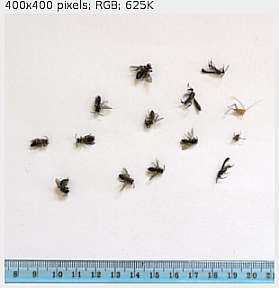
\includegraphics[width=.39\linewidth]{gfx3/seg/segb-1}} \
\subfloat[Insects in flight.]{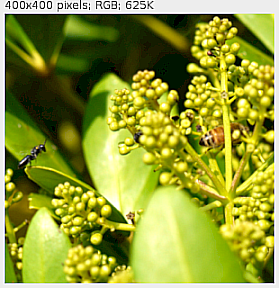
\includegraphics[width=.39\linewidth]{gfx3/seg/sega-1}}\\
\subfloat[8-bit grey scale image.]{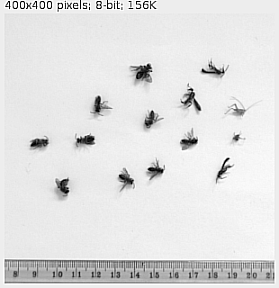
\includegraphics[width=.39\linewidth]{gfx3/seg/segb-2}} \
\subfloat[8-bit grey scale image.]{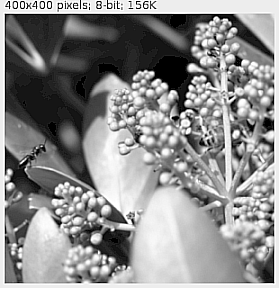
\includegraphics[width=.39\linewidth]{gfx3/seg/sega-2}}\\
\subfloat[Binary image.]{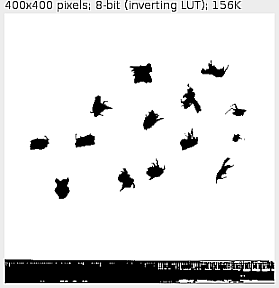
\includegraphics[width=.39\linewidth]{gfx3/seg/segb-3}} \
\subfloat[Binary image.]{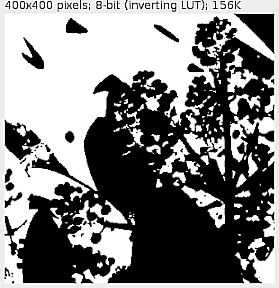
\includegraphics[width=.39\linewidth]{gfx3/seg/sega-3}}\\
\subfloat[Bimodal histogram.]{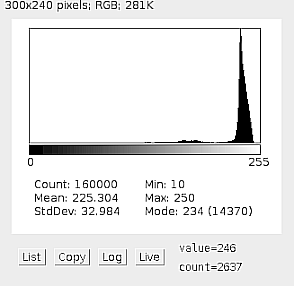
\includegraphics[width=.39\linewidth]{gfx3/seg/segb-4}} \
\subfloat[Multimodal histogram.]{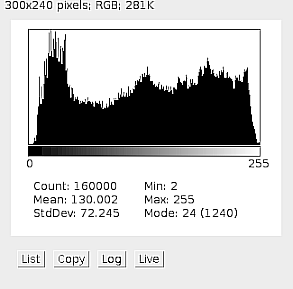
\includegraphics[width=.39\linewidth]{gfx3/seg/sega-4}}\\
\caption[Simple and difficult segmentation tasks.]{Examples of simple and difficult segmentation tasks. The images of (a) insect collections and (b) insects in flight. There is no single threshold values for the images of insects in flight; indicated by the multimodal histogram (h).}\label{fig:seg-binary}
\end{figure}

If images are not easily segmented, there are some alternative approaches. Frequently, there are other characteristics that define an image, such as connected structures, outlines, areas or textural qualities. For example, two alternative methods are edge detection, and region merging. \emph{Canny-Deriche filtering} \cite{Deriche1987} is a popular edge detection method. The $\alpha$ parameter controls the degree of smoothing applied where the default value is 1.0. Greater values suggest less smoothing, but more accurate detection; lower values suggest more smoothing but less accurate detection. Another technique is \ac{SRM}. It is a region-based method and it performs well on a range of images \cite{Nock2004, Nock2005}. $\emph{Q}$ -- the setting determining the approximate number of regions to segment. The algorithm examines one region per pixel and applies a statistical test on neighbouring regions in ascending order of intensity differences, to test if the mean intensities are sufficiently similar enough to be merged. Segmented regions can be represented by mean grey values as shown, or by index of the regions. Nock and Nielsen \cite{Nock2004, Nock2005} explain the \ac{SRM} is a very fast segmentation algorithm which copes well with noise and occlusions \cite[pg.1458]{Nock2004}. 

\subsubsection{Trainable segmentations}\label{sec:trainable-segmentations}
In most analyses \emph{any} aspect of the imaging pipeline can be tweaked to accommodate image characteristics or to highlight the key data required for specific analysis applications. However, few traditional techniques can be used on highly variable images, since methods cannot be applied to generalise over a wide range of pixel intensities. In this circumstance, machine learning techniques are far more effective. It is also the basis for the growing tendency towards using machine learning in challenging imaging tasks, as proposed by Ljosa and Carpenter \cite{Ljosa2009}.

Trainable image segmentation techniques work by utilising human visual knowledge to provide a machine learning algorithm with a set of \emph{expertly labelled examples}. For example, in Fiji the \ac{TWS} plug-in \cite{Kaynig2010} requires a user to provide two sets of labels. \ac{ROI} tools are used to select pixels samples belonging to foreground (class 1) and background (class 2) objects. Filters are applied to original image data and used to create a separate \emph{features stack}. In \ac{TWS} a user may select any combination of filters from a possible twenty; they can be grouped according to their main filter functions as shown in Table \ref{tab:tws-features}. During the learning process an machine learning algorithm uses the examples provided, and the features stack, to construct a purpose built classifier. The classifier can be used to segment similar types of images, including the one it was trained on. It is ambitious to ascertain what combination of image features best describes key objects, therefore some aspects of classifier training are  subjective. There are also a number of other confounding decisions to consider before applying machine learning for image segmentations. However, providing a user selects appropriate representative pixel samples and chooses filters that will provide a rich features stack for the analysis, machine learning algorithms work very well and can surpass other methods. Especially on challenging imaging problems.

\section{Trainable Weka Segmentations}
Machine learning options work well for studies that depend on variable images which are difficult to segment using conventional techniques. Outdoor imaging applications, off-the-shelf camera equipment and \ac{JPEG} compression are factors that impact image quality -- a topic which was briefly introduced in Section \ref{}. New tools that can mitigate the affects of poor quality images and have resulted in some innovative solutions for a diverse range of applications, from Johansson's \cite{Johansson2011} novel small vessel detection study, to the \ac{UAV} flood mapping system proposed by Feng et al. \cite{Feng2015a,Feng2015b}.

\begin{table}[!htbp]\myfloatalign \caption[Interactive segmentation method.]{Interactive segmentation method with \ac{TWS}.}\label{tab:tws-general} 
\begin{tabular}{lp{3.9in}}\toprule
1 & Select a minimum of two traces -- representing two classes.\\
2 & Train the base classifier and check output image.\\
3 & Tune classifier by selecting incorrectly segmented pixels: \\
& \ \ \ \ \ \ a) Assign pixels to the correct classes for re-classifying. \\
& \ \ \ \ \ \ b) Train final classifier. \\
4 & If segmentation is satisfactory then apply to all other \emph{similar} images.\\
5 & OR optimise classifier to reduce errors, increase processing speed by adjusting the: \\ 
& \ \ \ \ \ \ a) Features provided.\\
& \ \ \ \ \ \ b) Classifier type. \\
& \ \ \ \ \ \ c) Tuning parameters. \\
& \ \ \ \ \ \ d) Training set-up. \\
\bottomrule
\end{tabular}
\end{table}

The \ac{TWS} plug-in was designed for pixel level segmentation via semi-supervised learning primarily aimed towards biomedical imaging applications. As previously outlined, a user selects a set of features (e.g. such as edge detectors, texture filters) and using ROI tools, interactively selects pixel traces representing at least two classes. When classifier training is initiated the features of the input image will be extracted and converted to a set of vectors of float values, the format expected for Weka classifiers. Based on the samples provided a classifier is trained returning a segmented image, shown as a semi-transparent overlay corresponding to the class colours. The process is normally repeated until satisfactory segmentations are obtained. Good segmentation results are typically achieved over two training sessions, so the process is iterative and interactive. The time taken to train and classify data can range, depending on the image size, the amount of features selected, the chosen classifier and the number of cores of the processing machine. The default classifier is the \emph{FastRandomForest}. The algorithm is a multi-threaded version of random forest which is initialised with 200 trees and 2 random features per node. There are also five default training features (from a possible twenty), automatically set which include: Gaussian blur, Hessian, Membrane projections, Sobel filter and Difference of Gaussians. 

The general procedure used for classifier training in \ac{TWS} is outlined in Table~\ref{tab:tws-general}. Most training consists of a least two runs. The first returns broad segmentations as shown in  The second training run is optimised by selecting a few previously miss-classified ROI areas for re-classification. The main concept is to supply the \ac{RF} classifier with only a very small representative sample of classes. This enables the classifier to \emph{learn} to recognise, rather than \emph{memorise} target pixels\footnote{The concept of over-training is}. When the results of classifications are satisfactory it is possible to save a fully constructed classifier for use in other similarly related tasks.\ac{TWS} provides both the option to save as a standard Weka model file or immediately apply a constructed classifier via the \ac{GUI}. As described previously, all the training annotations can also be saved as an arff file. The file contains all the feature vectors derived from the pixels, belonging to each trace during training. During classification on new previously unseen images, the classifier can also be re-trained to incorporate new information based on other images and saved. 

\begin{figure}[!htbp] \myfloatalign
\subfloat[Stack of 16 images.]{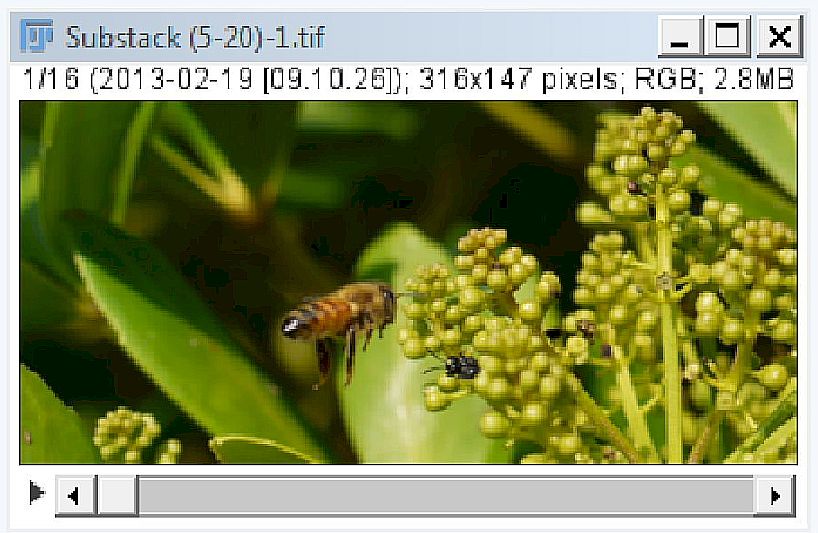
\includegraphics[width=.40\linewidth]{gfx3/rf/rf-tws1}}
\subfloat[Feature stacks.]{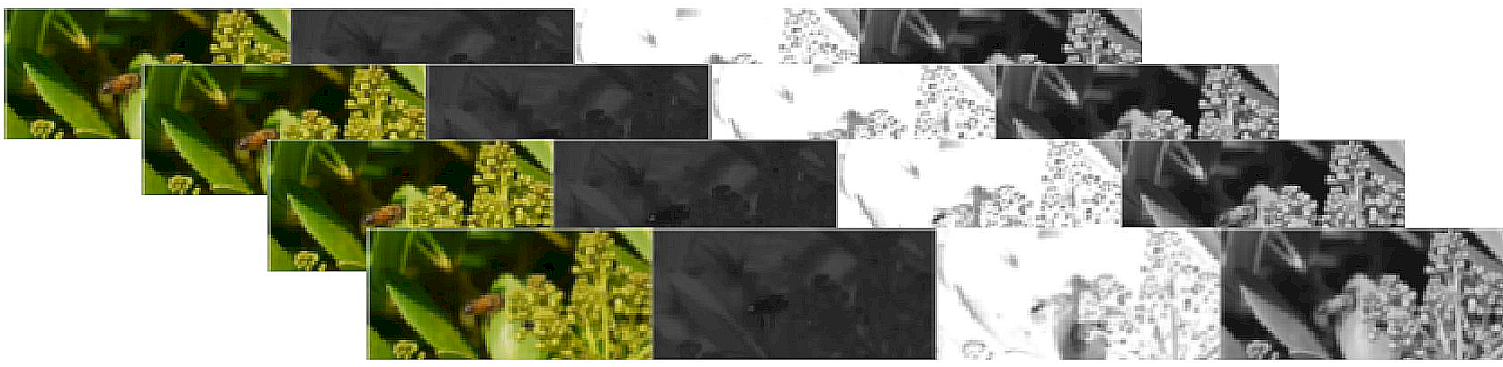
\includegraphics[width=.40\linewidth]{gfx3/rf/rf-tws2}}\\
\subfloat[Trainable weka segmentation procedure using a \ac{RF} classifier.]{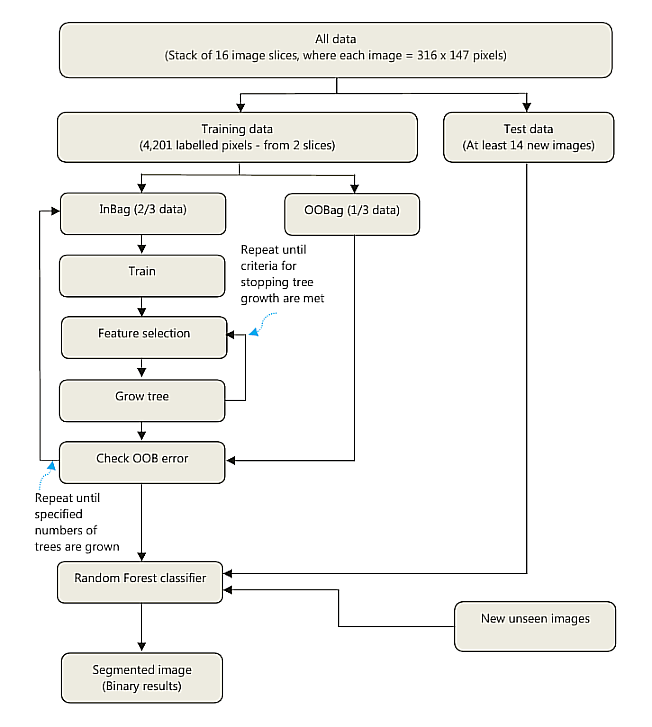
\includegraphics[width=1\linewidth]{gfx3/rf/rf-tws3}}\\
\caption[Trainable segmentation procedure.]{Trainable segmentation procedure using an \ac{RF} classifier. An \ac{RGB} stack of 16 (a) images are used to build the model; features stacks are constructed for each image slice (b). Sample traces are interactivity selected by a user to train the \ac{RF} classifier using the flowchart outlined in (c).}\label{fig:rf-tws}
\end{figure}

The default classifier in the \ac{TWS} workbench is the \ac{RF}. However, there are at least fifty other \ac{Weka} classifiers available. Each machine learning algorithm is equipped with a set of parametrisation tools. These settings are used to tune the classifiers for specific tasks. It is also possible to custom design \ac{Weka} classifiers and create new models for specific applications. Machine learning is a popular area of research is rapidly evolving as more algorithms are developed each year. Traditionally, support vector machines and neural networks were considered state-of-the-art. They have been used very successfully in a range of classification applications using real-world data. Until recently, no other machine learners have surpassed the performances of support vector machines or neural networks.

But according to a recent study by Fernandez et. al. \cite{Fernandez2014} the \acp{RF} are most likely to perform the best. Fernandez et. al. \cite{Fernandez2014} evaluated 179 classifiers from 17 families of learners. They undertook comprehensive evaluations by implementing the classifiers in Weka, R, C and Matlab; using the whole UCI data base\footnote{https://archive.ics.uci.edu/ml/datasets.html} (121 data sets). Their objectives were to determine which of the classifiers were most likely to perform the best on \emph{any} data set. The results were extensively reported, covering all aspects of classifier optimisations data set partitioning, and test configurations. Concluding that three out of the five best classifiers were from the random forest family, closely followed by support vector machines, neural networks and boosting ensembles.

A range of other studies have reported the on benefits of \acp{RF}. They continue to be developed and used in a range of seemingly unrelated applications. For instance, \ac{RF}'s have been applied to studies in: astronomy \cite{Albert2008}, biomedical imaging \cite{Genuer2010}, economic forecasting \cite{Kumar2006}, genetics \cite{Diaz2006}, pharmacology \cite{Svetnik2004}, species identification \cite{Larios2010}, ecological modelling \cite{Prasad2006,Cutler2007,Schwartz2006}, remote sensing for land-cover classification \cite{Rodriguez2012}, carbon mapping \cite{Mascaro2014}, forest classification \cite{Mellor2013}, \ac{UAV} flood mapping \cite{Feng2015a,Feng2015b} and invasive species mapping \cite{Cutler2003,Lawrence2006}. The breadth and range of studies suggests the \ac{RF} is a flexible all-round classifier suited to a range of natural real-world data. However, the study by Fernandez et. al. \cite{Fernandez2014} is the first to properly quantify the performances of \ac{RF} classifiers. It is likely the developers of \ac{Fiji} and \ac{TWS} selected the \ac{RF} classifier as the default model, based on anecdotal evidence of segmentation performances in a range of biomedical imaging applications. 

\section{Verification methods}\label{sec:verification-methods}
In contrast to other machine learners, the \ac{RF} algorithm has an internal error mechanism. The \ac{RF} takes a bootstrap of all the data provided for training. During construction, individual training sets for each tree are generated from the original set using sampling with replacement. The samples, which are not chosen for training, are called the out of bag samples. They are used to calculate the out of bag error ($ oo_{b} $) which is an unbiased estimate of the generalisation error. In contrast to other classifiers there is no need to perform cross-validation tests to get an unbiased estimate of the true test set error. 

In machine learning research, other parameters can be used to help determine the predictive accuracy of a classifiers. These typically include the overall number of correctly classified instances -- often in the form of a confusion matrix, the number of true positives and negatives, precision, recall, and the F-measure. Even a trivial classifier that incorrectly predicts every case as the target class can still achieve a high accuracy so it important to use appropriate performance measurements. Classifiers constructed using natural images can be more difficult to measure and this is more so if training datasets are skewed or unbalanced. When data is unbalanced the Kappa statistic is more informative because it is a \emph{chance-corrected} measure of agreement between classifications and true classes \cite{Di2004}. The statistic is calculated by taking the agreement expected by chance away from the actual observed agreements, and dividing this value by the maximum possible agreement as follows:

\begin{equation}
\kappa = \dfrac{P(A)-P(E)}{1-P(A)} \label{eq:kapa}
\end{equation}

Where $ P(A) $ is the observed agreement and $ P(E) $ is the expected agreement. The values of $\kappa$ are constrained to the interval $[-1, 1]$. A value of $\kappa = 0$ indicates a complete absence of agreement and $\kappa = 1$ shows a very strong agreement. Any value above zero indicates the classifier is, at the very least, performing better than by chance alone.

In many applications segmentation metrics give more insight, since they indicate how well images are partitioned into categories \cite{Jain2010,Jain2010a}. This is an important consideration for biomedical imaging problems since most performance measures are based on visual-image checks using ground-truth techniques. Until recently, classifier performance has been a subjective measure. As Unnikrishnan et al. \cite{Unnikrishnan2007} point out, "...the evaluation of segmentation algorithms thus far has been largely subjective, leaving a system designer to judge the effectiveness of a technique based only on intuition and results in the form of a few example segmented images. This is largely due to image segmentation being an ill-defined problem? There is no unique ground-truth segmentation of an image against which the output of an algorithm may be compare." \cite[pg. 929]{Unnikrishnan2007}.
Biomedical imaging method more frequently employ three quantitative segmentation metrics. They include the Pixel, Rand and Warping errors. For image segmentation analysis the ideal metrics for machine-human disagreement should tolerate minor differences in boundary location, penalise topological disagreements, and serve as a cost function for supervised learning \cite{Jain2010,Jain2010a}. The three metrics are defined as:

\begin{enumerate}
\item \emph{Pixel Error}: the squared Euclidean distance between the original and resulting images. 
The lower the error, the greater the agreement is between images. 
\item \emph{Rand Error}: the measurement of similarity between clusters of pixels. The lower the error the greater the agreement is between images. 
\item \emph{Warping Error}: Warping Error: A measurement that penalises topological disagreements and is used as a direct cost function of segmentations. The lower the error the greater the agreement is between images. 
\end{enumerate}

\section{Data management tools}
Database design are becoming vital components for research involving big data analysis. Sharing protocols are well established in some disciplines such as genomics, astronomy and meteorology, therefore substantial care is afforded to database design and access. But the shift towards more open models have not been adopted by all disciplines \cite{Soranno2015}. Similar points have been discussed previously in relation to the use of big data\cite{Hampton2013} and the slow adoption of automated image analysis \cite[p.12]{Gaston2004}. Data sharing is not always considered virtuous \cite{Lindenmayer2013} and some authors suggest paradigms are slow to change for some disciplines \cite{Evans2011,Hampton2013,Mascaro2014}. However, the progress towards open access, open-source and data sharing well advanced a range of interdisciplinary life science disciplines, which can provide good examples to follow \cite{Reichman2011,Steiniger2009}.

For example, the \ac{KNB} provides the facilities to store, share, discover, access and interpret complex ecological data and can be integrated with the open-source statistical package R, or used with a desktop application Morpho which allows users to create metadata for describing data in a standard format, and to search, edit or view data collections. There are a range of generic options which can be used to store data online, for example, cloud storage such as Dropbox \footnote{https://www.dropbox.com/} can be used for single users or OpenStack \footnote{http://www.ubuntu.com/cloud/ubuntu-openstack} for large distributed community developments \cite{Platforms2012}. Github is also a popular repository for collaborative project developments and code design. While it was not specifically designed for sharing data it is used to as centralised hub for smaller research projects \cite{Easlon2014, Altermatt2014}.

\section{Review summary}\label{sec:ch3-review-summary}
\begin{remark}{The imaging method}
Delaney \cite{Delaney2008} writes, "from the earliest days of the photograph to the present, its value has been recognised by the scientific community to help them document and understand the natural world." \cite[pg.76]{Delaney2008}.
\end{remark}

Given the variety and complexity of some machine learning algorithms, and the overall objectives of this thesis, there were few reasons to examine the performances of other classifiers or investigate the internal workings of the \ac{RF} classifiers. Both lines of these investigations would have quickly led into the areas of machine learning and statistical analysis, which are beyond the scope and expertise of this research. Rather, when taken on the whole, it was difficult to look past the evidence indicating the \ac{RF} model would be a good tool for the segmentation tasks associated with the image-centric bee monitoring system.

The performance characteristics of \ac{RF} classifiers can be internally measured during run-time, externally assessed or compared in Weka using statistical tools such as a confusion matrix, or quantified using segmentation metrics.
